The standard model of particle physics (SM) describes the fundamental particles and interactions between them. It is a theory that successfully predicted the existence of several at that time undiscovered particles like e.g. the W boson \todo{Quellen: Teilchen Entdeckungen}, the top quark or the $\tau$ neutrino. In addition, it has been tested extensively in electroweak precision measurements at LEP. \\
Although the SM shows so far a remarkably successful performance there are also some open questions which can not be answered within the SM. Thus several theories have been developed to address problems which go beyond the SM. One of such well-motivated extensions is supersymmetry (SUSY) for which however no experimental evidence has been found so far. \\
After a short introduction to the phenomenology of the standard model including a discussion of specific shortcomings~\cite{bib:PDG:2012}, the basic concepts of supersymmetry are introduced in this chapter \todo{Ref?}. In addition, general concepts of searches for supersymmetry at collider experiments are discussed together with a summary of the current status of the results of such searches which have been performed in the past.
\section{The Standard Model of Particle Physics}
\label{sec:sm}
The description of the SM comprises the elementary particles and their interactions. In general, one distinguishes between two types of particles: fermions and bosons. While matter particles are fermions with half-integer spin, the fundamental forces are mediated via bosons carrying integer spin. An overview of the contents of the SM is given in Fig.~\ref{fig:SM} where the particles are denoted together with their interactions \footnote{Gravity is not included in the current representation of the standard model and thus it is not discussed in this thesis.}. \\
\begin{figure}[!tp]
  \centering
  \begin{tabular}{c}
    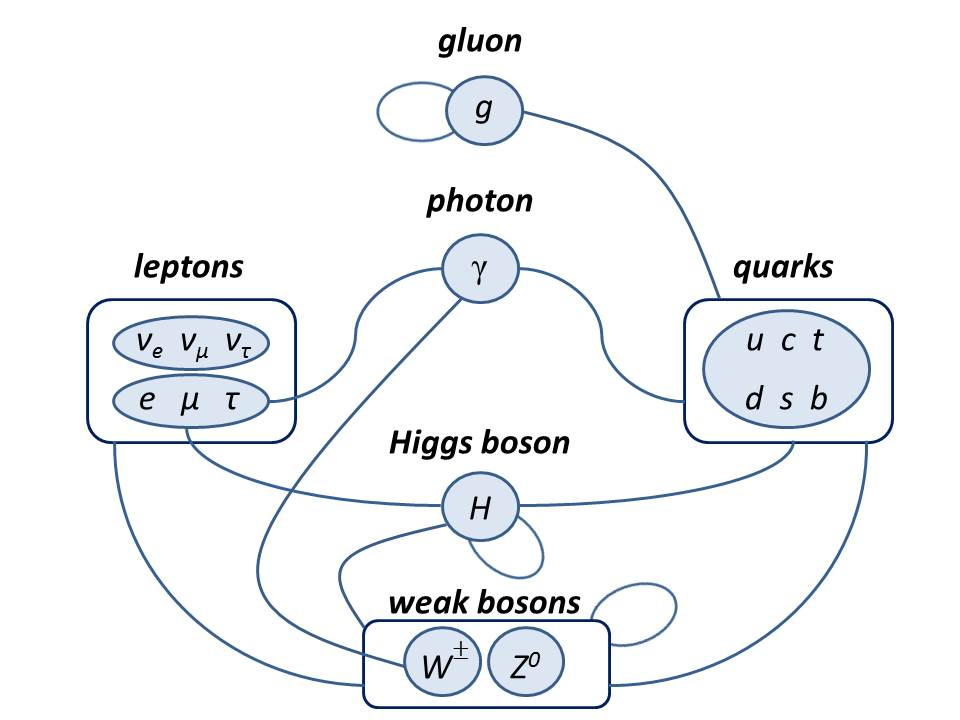
\includegraphics[width=0.9\textwidth]{figures/SM.jpg}
  \end{tabular}
  \caption{Overview of particles contained in the standard model. Blue lines indicate interactions between different particles.}
  \label{fig:SM}
\end{figure}
Mathematically the standard model is a quantum field theory where interactions between particles are described via gauge symmetries. The underlying gauge group of the standard model is 
\begin{equation*}
SU(3)_{C} \otimes SU(2)_{L} \otimes U(1)_{Y}
\end{equation*}
where $SU(3)$ is the gauge group of the strong force and $C$ indicates that this force acts on the colour charge, $SU(2)$ represents the weak force and $L$ denotes that this force only acts on left-handed fermions, while $U(1)$ represents the electromagnetic force acting on the hypercharge $Y$.\\
A brief description of the properties of the particles contained in the SM and the corresponding interactions is given in the following:
\begin{description}

\item \textbf{Matter Constituents:}
In the SM, one distinguishes between twelve different fermions being the elementary constituents of matter. For each fermion there exists also an antiparticle which carries the opposite signed quantum numbers.
 \begin{description}
  \item \textit{Leptons:} The SM contains in total six leptons which are three negatively charged leptons (\lel, \lmu, \ltau) and three neutral leptons (\nue, \numu, \nutau), the neutrinos. In addition to the charge, leptons are also distinguished according to the lepton numbers which are electron number $L_{\lel} = 1$ for electron and electron-neutrino, muon number $L_{\lmu} = 1$ for muon and muon-neutrino and tauon number $L_{\ltau} = 1$ for tauon and tauon-neutrino. Each pair of lepton and neutrino carrying the same lepton number is forming a so-called \textit{generation} where \lel and \nue belong to the first generation, \lmu and \numu to the second and \ltau and \nutau to the third, respectively.
  \item \textit{Quarks:} The remaining six fermions in the SM are quarks and can be grouped into generations analogous to the leptons. The first generation is populated by up- and down-quark (\qu, \qd), the second by charm- and strange-quark (\qc, \qs) and the third by the top- and bottom-quark (\qt, \qb). All quarks carry electrical charge but different than for leptons it is not integer but $+2/3$ for the up-type quarks (\qu, \qc, \qt) and $-1/3$ for down-type quarks (\qd, \qs, \qb). Besides to the electrical charge, quarks also carry color charge which comes in three types.
 \end{description}
In addition to the attributes described above, fermions are furthermore characterized by the weak isospin. Left-handed fermions in each generation form an isodoublet with a weak isospin of $\pm 1/2$ while right-handed components are isosinglets with a weak isospin of 0. 
\item \textbf{Fundamental Forces:}
Matter particles interact with each other through fundamental forces mediated via gauge bosons. These bosons arise from the principle of local gauge invariance under symmetry transformations. 
 \begin{description}
  \item \textit{Electromagnetic Force:} The description of the electromagnetic force is based on the theory of \textit{Quantum Electrodynamics} (QED). It is communicated between electrically charged particles, like the charged leptons and quarks, by the exchange of photons. These are massless and electrically neutral resulting in the property that the electromagnetic force is long ranged.
  \item \textit{Weak Force:} The weak force acts on the weak charge which is carried by all fermions in the SM. It is mediated by three vector bosons -- namely the two charged \Wpm bosons and the neutral \Z boson. These bosons are unlike the photon massive with masses of $\Wpm = 80.385 \pm 0.015$\gev and $\Z = 91.1876 \pm 0.0021$\gev~\cite{bib:PDG:2012}. As a result the weak interaction is suppressed with respect to the electromagnetic force. \\
Weak interactions preferably take place within one generation, e.g. \lel or \lmu transform into the respective neutrinos when emitting a \Wm. However, since the mass eigenstates in the weak interaction differ from the flavour eigenstates, \Wpm bosons can also couple to fermions between different generations. In the quark-sector typically a representation is chosen where the up-type flavour eigenstates correspond to the mass eigenstates and the down-type quarks mix. This mixing is described by the CKM-matrix \todo{Quelle}. This is an unitary matrix, described by three mixing angles and one CP-violating phase, which indicates the relative strength between individual transitions. 
  \item \textit{Strong Force:} The theoretical framework describing the strong force is called Quantum Chromodynamics (QCD) \todo{Quelle}. It is mediated via eight massless gluons and acts on the colour charge which is carried for instance by quarks. In contrast to the photon which is electrically neutral and thus can not interact with itself, gluons carry a colour charge and hence are able to couple to themself. The colour charge exists in three different states commonly denoted as 'red', 'green' and 'blue'. Quarks and gluons are collectively referred to as partons. \\
Regarding the dependence on the distance the strong force behaves differently than other fundamental forces: the coupling strength increases with rising distance. This is a consequence of the different colour states and the self-coupling property of gluons. It is usually referred to as \textit{confinement} and causes the effect that coloured objects can not exist freely. In fact when separated, coloured objects start to build new coloured particles until only a colour neutral formation is left. Such colourless objects linked by the strong force are named hadrons. On the other hand, particles taking part in the strong interaction start to behave quasi-free when they are brought close together. This feature is known as \textit{asymptotic freedom}.   
 \end{description}
First proposed by Salam, Glashow and Weinberg \todo{Quelle}, the electromagnetic and the weak force could be successfully unified into the electroweak force. As denoted earlier, the weak force acts on the weak isospin $T_{3}$ while the electromagnetic force acts on the hypercharge $Y$. These two quantities are connected via the following relation to the electric charge $Q$
\begin{equation*}
Q = T_{3} + Y/2
\end{equation*}
In the electroweak theory, three gauge bosons $W^{1,2,3}_{\mu}$ are introduced for $SU(2)_{L}$ and one gauge boson $B_{\mu}$ for $U(1)_{Y}$. The physical states photon, \Wpm and \Z are formed by mixing of these massless states. While the charged $\Wpm_{\mu}$ bosons are superpositions of $W^{1}_{\mu}$ and $W^{2}_{\mu}$, the fields $A_{\mu}$ of the photon and $Z_{\mu}$ of the neutral vector boson are obtained by a mixing of the gauge fields $W^{3}_{\mu}$ and $B_{\mu}$ parametrized by the weak mixing angle $\theta_{W}$ \todo{Formel?}.  
\item \textbf{Higgs Boson:} The electroweak theory in the current representation requires that fermions and bosons are massless particles as mass terms violate the gauge invariance under $SU(2)_{L} \otimes U(1)_{Y}$ transformations. This is in contradiction to experimental observations which have shown that all particles, except for photon and gluon, in fact have mass. \\
An explanation for the generation of particle masses without violation of the principles of the electroweak theory is provided by the \textit{Higgs-mechanism} \todo{Quellen} which is based on the concept of spontaneous symmetry breaking. The main idea behind this meachnism is that in general the principle of local gauge invariance is obeyed, but that it is explicitly broken by the ground state. In the context of the Higgs-mechanism this is realized by the introduction of the Higgs field described by a potential with a non-zero minimum value \todo{Formel?}. This non-vanishing minimum represents the expectation value of the quantum field in the vacuum -- the vacuum expectation value. The masses of particles are eventually generated by the couplings to the Higgs field. \\
Furthermore, the Higgs-mechanism also predicts the existence of a new heavy boson, the Higgs boson, which is a quantum excitation of one of the components of the Higgs field. It is supposed to be a scalar and the Higgs mass one of the free parameters of the SM. \\
The discovery of a new boson at a mass of around 125~\gev has been announced by the ATLAS and CMS collaborations in 2012 \todo{Quelle}. As all properties of this new boson are consistent with SM predictions so far \todo{Quelle}, this indicates that the last existing gap of the SM could finally be closed. 
\end{description}

\subsection{Limitations of the Standard Model}
\label{subsec:sm_shortcomings}
Although the SM has been incredibly successful so far and lead to several discoveries while withstanding numerous precision tests, it is known to be on the other hand also an incomplete theory. Some of known shortcomings of the SM are discussed in some detail in the following.
%As stated earlier it is e.g. not possible to include gravity at the moment or provide an explanation for the observed matter-antimatter asymmetry in the universe. These are only some of known shortcomings of the SM of which a few additional ones are discussed in some detail in the following.
\begin{description}
\item \textbf{Gravity:} As stated already earlier, the SM contains no description of gravity. In particular, it is currently not possible to unify general relativity and quantum theory in one common concept.
\item \textbf{Matter antimatter asymmetry:} According to the SM matter and anitmatter exist to equal amounts in the universe which is in fact not the case. A theory which would be able to explain such an asymmetry needs some source of CP-violation. The only source of CP-violation within the SM is arising from the CKM matrix as described in~\ref{sec:sm}. However, this is not enough to be able to explain the degree of matter antimatter asymmetry in the universe \todo{Quelle}.   
\item \textbf{Unification of couplings:} The unification of the electromagnetic and the weak force leads to the question, if it is even possible to further unify the electroweak force with the strong force in order to build a combined theory usually referred to as Grand Unified Theory (GUT). This would imply that the coupling constants of the SM intersect when extrapolating them from the electroweak to the GUT scale. However, this feature is not observed within the SM.
\item \textbf{Origin of dark matter and dark energy:} There exist several cosmological observations that indicate that the matter described by the SM makes up only around ... \% of the universe \todo{Quelle}. A by far larger part of ... is assigned to so-called \textit{dark matter} which is presumably neutral and only weakly interacting. The only particles within the SM possessing such attributes are neutrinos. However, they are not able to account for the whole relic density present in the universe \todo{Quelle}. Furthermore, for the major part of the universe making up .. \% there is no hint at all what its' nature could be. Thus it is typically denoted with \textit{dark energy}.
\item \textbf{Hierarchy problem:} The observable mass of the Higgs boson is given by the bare mass of the Higgs boson plus contributions arising from higher order corrections caused by each massive SM particle. These higher order corrections are usually dependent on an ultraviolet cut-off scale \todo{Formel?}. Conventionally this UV cut-off scale is chosen to be the Planck scale. This would result in a Higgs mass considerably larger than the oberserved mass of around 125~\gev and requires an enormous amount of fine tuning in order to address this problem. 
\end{description}

\section{Supersymmetry}
\label{sec:susy}
In order to overcome the weaknesses of the SM and to provide explanations for so far unsolved problems of which some have been dicussed in~\ref{subsec:sm_shortcomings}, several theories have been developed which go beyond the SM. Among those, a favoured extension is \textit{supersymmetry} (SUSY) as it is able to provide several benefits at once. In this section a brief introduction to the general concept of supersymmetry is given with focus on the \textit{Minimal Supersymmetric Standard Model} (MSSM). For details see ... .\\ 
\\
%The basic idea behind supersymmetry is that each standard model particle gets a supersymmetric partner particle which possesses the same quantum numbers except for the spin which differs by $1/2$. 
The basic idea of a supersymmetric theory is that a fermionic state is converted into a bosonic state and vice versa by the generator of a supersymmetry transformation $Q$ according to
\begin{equation*}
Q \ket{\mathrm{fermion}} \, = \, Q \ket{\mathrm{boson}}, \hspace{20mm} Q \ket{\mathrm{boson}} \, = \, Q \ket{\mathrm{fermion}}.
\end{equation*}
The supersymmetric fermionic and bosonic partner particles are called \textit{superpartner} and form together the irreducible representations of the supersymmetry algebra named \textit{supermultiplets} with the same number of fermionic and bosonic degrees of freedom. It can be shown \todo{Quelle} that in case of unbroken supersymmetry partner particles within one supermultiplet have the same mass as well as the same quantum numbers like electric charge, weak isospin and color degrees of freedom, except for the spin.\\
\\
Furthermore, in a general supersymmetric theory fulfilling the criteria of gauge invariance and renormalisability, processes are allowed violating either the lepton or baryon number conservation. However, such a process has not been observed experimentally so far and would imply for instance a rapid decay of protons. The current lower limit on the proton lifetime is ... \todo{Quelle} and indicates that such processes must be suppressed. In order to achieve this, a new quantum number called \textit{R-parity} is introduced according to
\begin{equation*}
R = (-1)^{3(B-L) + 2S}
\end{equation*}
with baryon number $B$, lepton number $L$ and spin $S$. It is a multiplicative quantum number and amounts to $R= +1$ for SM particles while it is $R = -1$ for supersymmetric particles. Assuming R-parity conservation no baryon or lepton number violation processes occur \todo{Quelle RPV SUSY in Fussnote} ~\footnote{There exist also several R-parity violating SUSY models which are not in contradiction to the observed proton lifetime. However, these are not subject of this thesis and thus not discussed.}. In addition, the assumption of R-parity conservation leads to further phenomenological implications:
\begin{itemize}
\item SUSY particles can only be produced in pairs at collider experiments as only even numbers of supersymmetric particles can occur in an interaction vertex.
\item The lightest supersymmetric particle (LSP) is stable and thus any decay chain of a supersymmetric particle finally ends in a state containing an odd number of LSPs.
\end{itemize}
A R-parity conserving supersymmetric theory as described above provides some elegant solutions to open questions as raised in section~\ref{subsec:sm_shortcomings}. As discussed there, the Higgs mass suffers from quadratically divergent contributions arising from higher order corrections caused by SM particles. However, since in SUSY each SM particle gets a supersymmetric partner these higher order corrections cancel as all supersymmetric particles contribute in an unbroken theory with equal size but opposite sign as their corresponding SM partner. Thus SUSY is able to provide a solution to the hierarchy problem. But the observation of such kind of supersymmetric particles with the exact same masses as their SM correpondents would have happened already. Since this is not the case, one knows from all experimental results that supersymmetry in fact has to be a broken symmetry. In order to still be able to provide a solution to the hierarchy problem, supersymmetric particles are expected to be not heavier than $\mathcal{O}(\mathrm{1\tev})$. This is the main argument why one would expect supersymmetric particles to be in the \tev range, well within the reach of the LHC. Especially the superpartner of the top quark is expected to be not too heavy in order to be able to cancel the contributions from top loops. This is necessary as these give the largest contributions since the top quark is the heaviest particle in the SM. \\
\begin{figure}[!tp]
  \centering
  \begin{tabular}{c}
    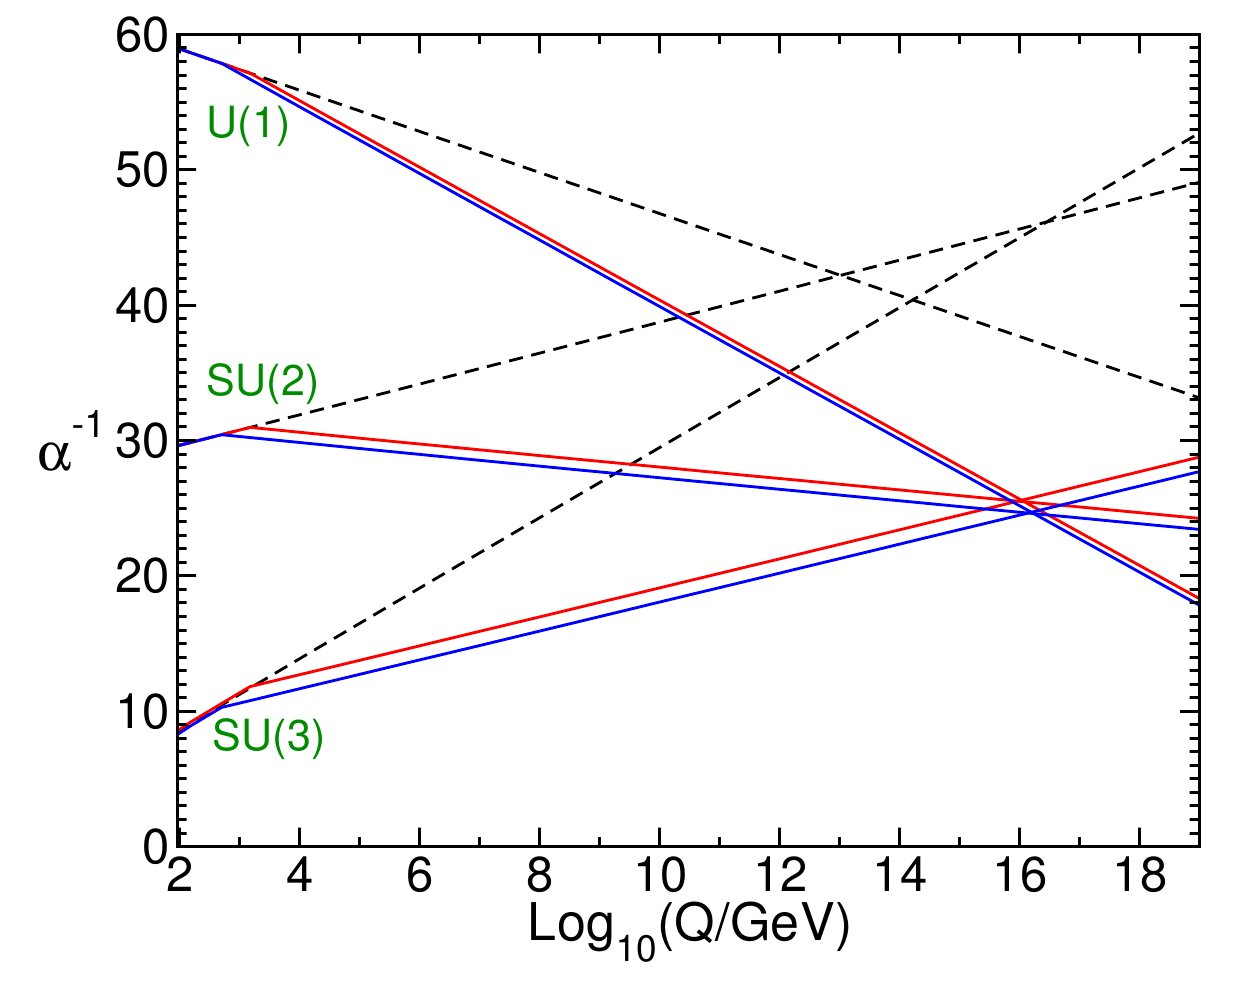
\includegraphics[width=0.75\textwidth]{figures/Couplings.jpg}
  \end{tabular}
  \caption{Comparison of the renormalization group evolution of the couplings $\alpha_{a}^{-1}$ in the SM (dashed lines) and the MSSM (solid lines) including two-loop effects. The masses of the supersymmetric particles in the MSSM are considered as a common threshold changing between 500\gev and 1.5\tev while $\alpha_{3}(m_{Z})$ is varied between 0.117 and 0.121. Taken from~\cite{Martin:1997ns}.}
  \label{fig:couplings}
\end{figure}
In addition to this naturalness aspects, the coupling constants of the forces which do not intersect within the SM actually meet in one point when extrapolating the couplings from the electroweak to the GUT scale considering the existence of supersymmetric particles. This effect is illustrated in Fig.~\ref{fig:couplings}. It is visible that the evolution of the couplings is modified with respect to the SM at that energy scale where the supersymmetric particles enter. In general, this hints to the possibility of a grand unification.\\
Besides the two advantages discussed above, R-parity conserving SUSY models also provide a suitable dark matter candidate. As discussed previously, each decay of supersymmetric particles finally leads to the existence of an LSP which can not decay further. Thus, it is an adequate DM candidate when it is electrically uncharged and only weakly interacting \todo{Quelle}.

\subsection{The MSSM}
\label{subsec:mssm}

\begin{table}[htbp] 
  \centering
  \label{tab:mssm_particles}
%   \makebox[\linewidth]{
    \begin{tabular}{cccc}
%      \hline
      \toprule
      Type & Spin & Gauge eigenstates & Mass eigenstates \\
      \midrule
      \midrule
      Higgs bosons & 0 & $H_{u}^{0}$ $H_{d}^{0}$ $H_{u}^{+}$ $H_{u}^{-}$ & $h^{0}$ $H^{0}$ $A^{0}$ $H^{\pm}$  \\
      \midrule
      & & $\tilde{u}_{L}$ $\tilde{u}_{R}$ $\tilde{d}_{L}$ $\tilde{d}_{R}$ &  see left \\
      Squarks & 0 & $\tilde{s}_{L}$ $\tilde{s}_{R}$ $\tilde{c}_{L}$ $\tilde{c}_{R}$  & see left \\
      & & $\tilde{t}_{L}$ $\tilde{t}_{R}$ $\tilde{b}_{L}$ $\tilde{b}_{R}$ & $\tilde{t}_{1}$ $\tilde{t}_{2}$ $\tilde{b}_{1}$ $\tilde{b}_{2}$ \\
      \midrule
      & & $\tilde{e}_{L}$ $\tilde{e}_{R}$ $\tilde{\nu}_{e}$ &  see left \\
      Sleptons  & 0 & $\tilde{\mu}_{L}$ $\tilde{\mu}_{R}$ $\tilde{\nu}_{\mu}$ & see left \\
      & & $\tilde{\tau}_{L}$ $\tilde{\tau}_{R}$ $\tilde{\nu}_{\tau}$ & $\tilde{\tau_{1}}$ $\tilde{\tau_{2}}$ $\tilde{\nu_{\tau}}$ \\
      \midrule
      Neutralinos  & 1/2 & $\tilde{B}^{0}$ $\tilde{W}^{0}$ $\tilde{H}_{u}^{0}$ $\tilde{H}_{d}^{0}$ & $\tilde{\chi}_{1}^{0}$ $\tilde{\chi}_{2}^{0}$ $\tilde{\chi}_{3}^{0}$ $\tilde{\chi}_{4}^{0}$ \\
      \midrule
      Charginos & 1/2 & $\tilde{W}^{\pm}$ $\tilde{H}_{u}^{+}$ $\tilde{H}_{d}^{-}$ & $\tilde{\chi}_{1}^{\pm}$ $\tilde{\chi}_{2}^{\pm}$ \\
      \midrule
      Gluino & 1/2 & $\tilde{g}$ & see left \\
      \midrule
      Gravitino & 3/2 & $\tilde{G}$ & see left \\
      \bottomrule
    \end{tabular}%}
 \caption{Supersymmetric particles contained in the MSSM neglecting mixing in the first two sfermion generations. Following~\cite{Martin:1997ns}.} 
\end{table}

\subsection{SUSY-Breaking}
\label{subsec:susy_breaking}

\subsection{Searches for Supersymmetry at Collider Experiments}
\label{subsec:susy_status}
SUSY is easy to search for at colliders. That is why we do it...bla bla bla bla bla

\begin{itemize}
\item how do we search at colliders?
\item searches at previous experiments
\item status: 7 TeV cmssm
\item cross sections at 8 tev
\end{itemize}
